\chapter{Spectroscopy of  a ws\textup{e}$_2$ gate device}\label{spectroscopy}

The goal of this thesis was the fabrication of gate-tunable \tmdg devices that show narrow spectral lines due to their encapsulation in \hbn. The so far best sample is a gate-structure made of tungsten-diselenide (\wse\!). The results of spectroscopic measurements on this sample are presented in this chapter. Its quality will be acessed by fitting peak functions to the spectral lines to find their linewidth. The same procedures are used to track the peak positions both at different charge densities and different magnetic fields to find $g$-factors of the spectral lines, that could help to identify their origin more precisely.

\section{Optical setup}\label{opticalsetup}

\begin{figure}
	\centering
	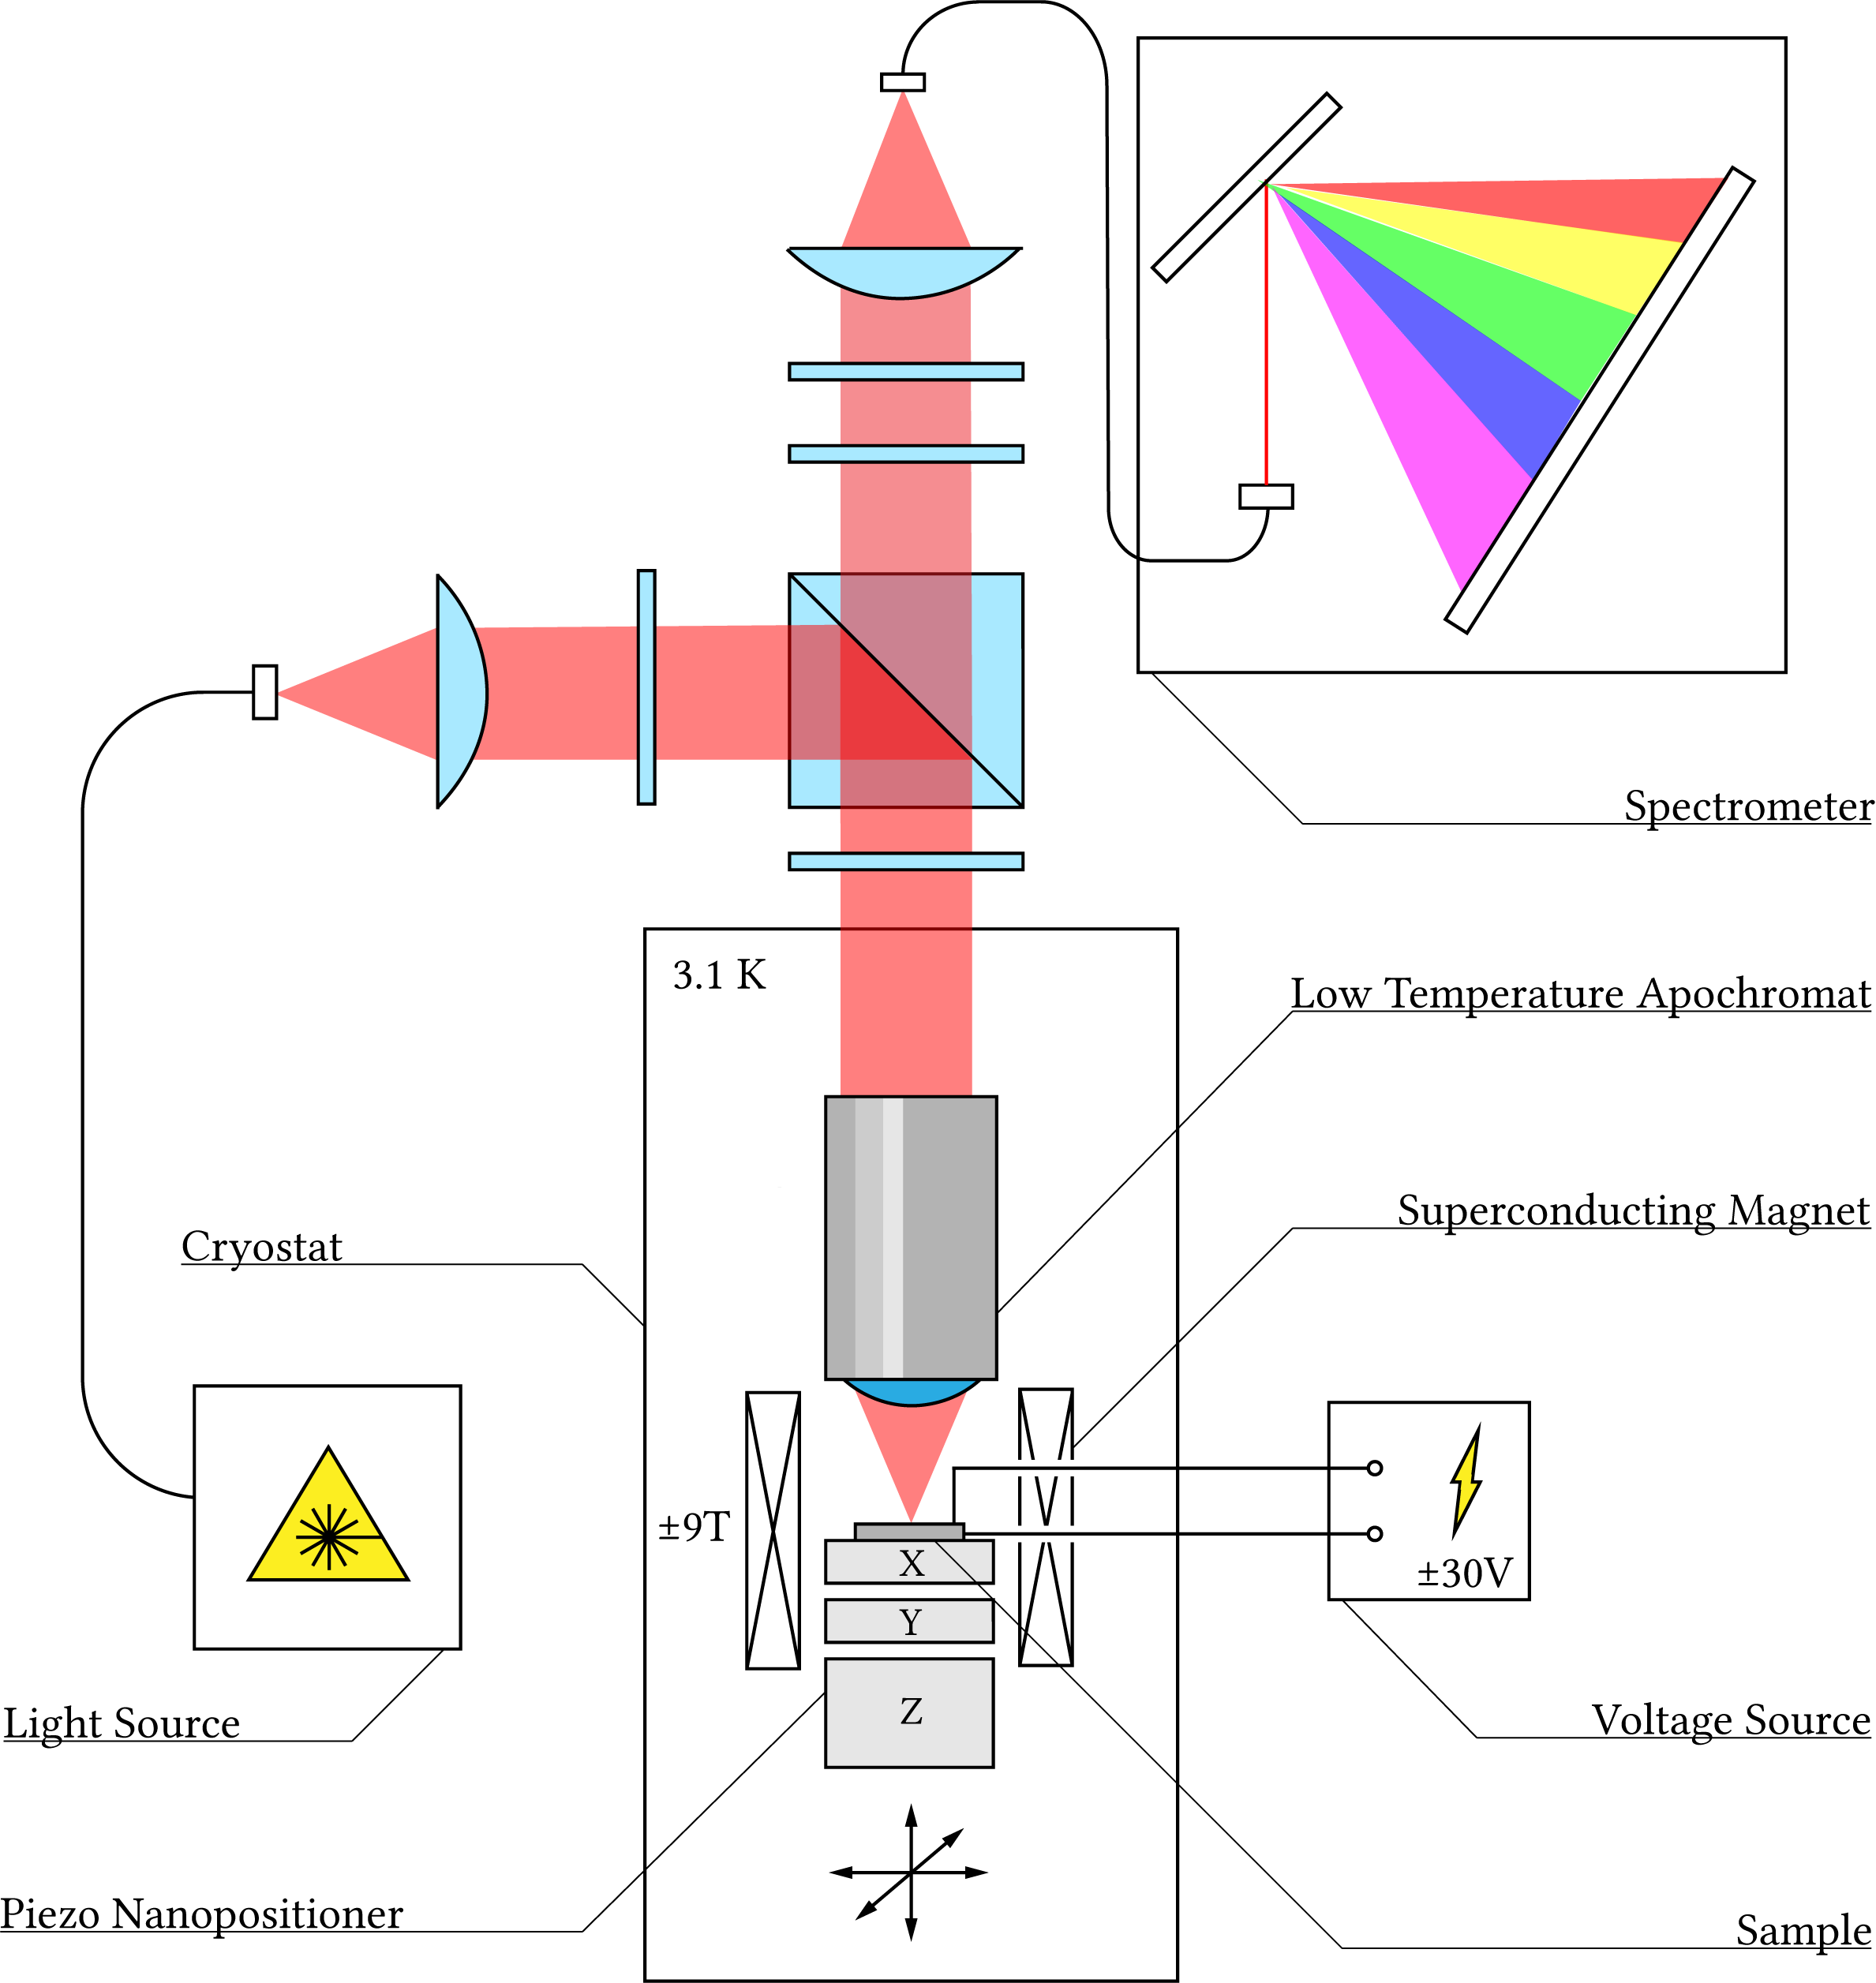
\includegraphics[width=.8\textwidth]{OptischerAufbau.png}
	\caption{Optical setup for confocal spectroscopy: Light from a \textbf{laser}-source is guided to the setup in a single mode opical fibre and collimated. To cut off raman-modes, that are created in the fibre a \textbf{shortpass} filter is installed behind the collimator. A \textbf{linear polarizer} defines a polarization axis. A \textbf{beam-sampler} is reflecting the excitation beam into a \textbf{low temperature apochromat}, whose focus lies on the sample, with a spotsize of \textasciitilde\- 0.5\mu m. The sample is mounted on a \textbf{piezo nanopositioner}, that is placed inside a \textbf{cryostat} at a temperature of up to 3.1 K or in a container of liquid helium at 4.2 K. The cryostat is equipped with a \textbf{superconducting magnet} that can supply a homogenious magnetic field up to 9 T. The sample electrodes are connected to a \textbf{voltage source} (Yokogawa) that supplies {\small$\pm$}32V. The detection spot is identical with the excitation. The reflection or photoluminescence is collimated again in the objective and passes through a $\sigma^-$/$\sigma^+$--analyzer consisting of a \textbf{quarter waveplate} and a \textbf{linear polarizer}, before being focussed in the detection fibre that connects to a \textbf{spectrometer}. A \textbf{camera} can be used to monitor the spot and image the sample, if it is brought out of focus.}
	\label{opticalsetup}
\end{figure}

\begin{figure}[t]
	\begin{subfigure}{0.49\textwidth}
		\caption{}
		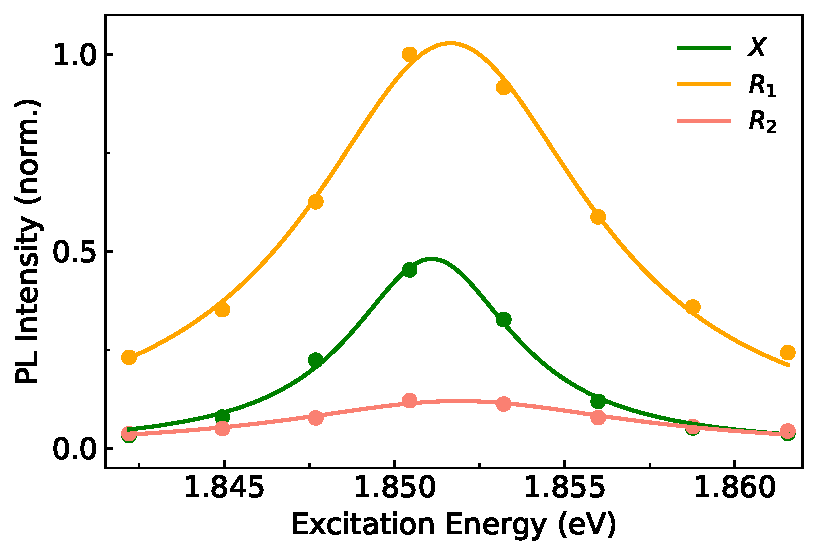
\includegraphics[width=\textwidth]{ple_2s}
	\end{subfigure}
	\begin{subfigure}{0.49\textwidth}
		\caption{}
		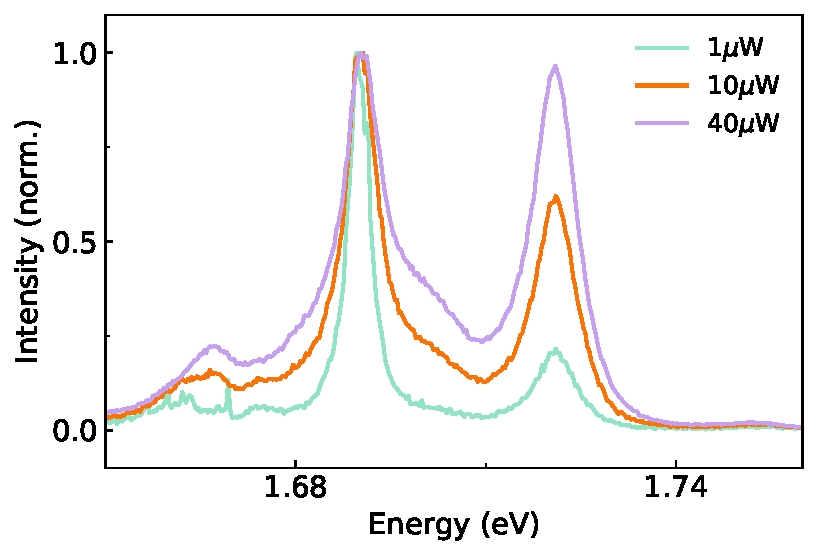
\includegraphics[width=\textwidth]{power}
	\end{subfigure}
	\caption{\textbf{A} Photoluminescence-excitation scan over the 2s resonance in \wse\!. To observe the complete spectrum, excitons have to be excited off-resonance. To create excitons as efficient as possible an excited exciton state, the 2s state can be pumped, that lies about 30 nm or 150 meV above the main exciton resonance. In this sample all spectral lines are at maximum intensity when pumped at 1.851 meV or 669.3 nm. \textbf{B} A higher excitation power means shorter integration times and higher signal to noise ratio but also boradens the spectral lines. For the $R_1$ peak the linewidth rose from 4.3 to 12.0 meV between 1--40 \mu W of excitation.} 
%8.9linewidth
	\label{optimum}
\end{figure}

The optical setup is a confocal microscope operated at cryogenic temperatures. This means that the sample is placed in the focal plane of a low temperature objective and insteat of capturing a wide field image of the sample only the signal from the focal point is collected. With a high quality objective the spot is only limited by the fundamental diffraction limit, yielding high spatial resolution. The other advantage is the high ratio between excitation power and collected signal, which extends the limits on integration time and thus the signal to noise ratio. A diagram of the complete setup can be seen in figure \ref{opticalsetup}. The excitation beam from a laser is guided to the so called excitation arm with a single mode optical fibre. It passes though a linear plolarizer to define a polarization axis and is reflected to the objective by a beam-sampler. To analyze circular dichroism in the detected beam, it passes through a quarter waveplate and another linear polarizer before being coupled into another optical fibre, that is connected to a spectrometer. The sample is mounted on a piezo nanopositioner inside a cryostat or a container of liquid helium and connected to a voltage source, that can tune the charge density in the \tmdg flake. A strong, homogenious magnetic field along the $z$-axis of the sample can be supplied by a superconducting magnet.

For \pl spectroscopy, the sample is excited by a laser beam with a narrow frequency profile and high power. The optimal parameters are determined by different factors. The optimal laser power depends on the obseved features. At a very low power emission from quantum dots can be observed, that saturate and bleach at a higher intensity---this is desirable in this case, as the observed spectrum should be as representative as possible. If the power is to high though, non-linear effects such as the formation of bi-excitons can start to play a role and the exciton emission saturates. Even before that the spectral linewidth of some peaks can rise significantly with the power, lowering the resolution of the spectrum (see figure \ref{optimum} \textbf{A}). Another problem of too high laser power is photoinduced doping, that counteracts the inetentional doping with an applied gate voltage\cite{wang_photoinduced_2016,cunningham_photoinduced_2017}. Therefore tuning to the negative regime only works for low excitation power. Even at low powers this beam has a much higher intensity, than the collected \textsc{pl} and has to be tuned to a higher frequency than the main exciton resonance, to obtain a complete spectrum without distrurbance from the excitation beam. To avoid stray light inside the spectrometer a longpass filter additionally blocks the laser before entering the detection fiber. A shortpass filter in the excitation arm blocks Raman modes of the optical fiber, a result from high excitation power, that can have frequencies overlapping with the \pl of the sample. Pumping off-resonance however results in a very inefficient ratio between excitation power and collected \pl\!. To still achieve a good signal-to-noise ratio, an excited state of the exciton---the 2s resonance---can be pumped (see figure \ref{optimum} \textbf{A}). While this resonance is much weaker than the main exciton resonance pumping at frequency still results in a signal of five times the intensity when compared to off-resonance excitation.
When the setup is operated for reflection spectroscopy these filters are omitted. Instead, the sample is illuminated with a broad band white light source at a low power. To find the signal, a background spectrum, recorded in absence of the \tmdg flake is substracted from the main spectrum.

\[ 
	S_R = \frac{\Delta R}{R} = \frac{R_{\mathrm{flake}} - R_{\mathrm{background}}}{R_{\mathrm{background}}}
\]

The signal $S_R$ is the difference of the Reflection signals of \tmdg flake and background. The division by the background reflection is made to normalize the signal. The resulting reflection spectrum should show only features, of the flake. In practice, the obtained data has to be evaluated with some precautions in mind, to avoid misidentifying for example interference effects due to differences in \hbng thickness as features of the absorption behavior of the sample.

\section{Modelling peak shapes}\label{fits}

\begin{figure}[t]
	\begin{subfigure}{0.49\textwidth}
		\caption{}
		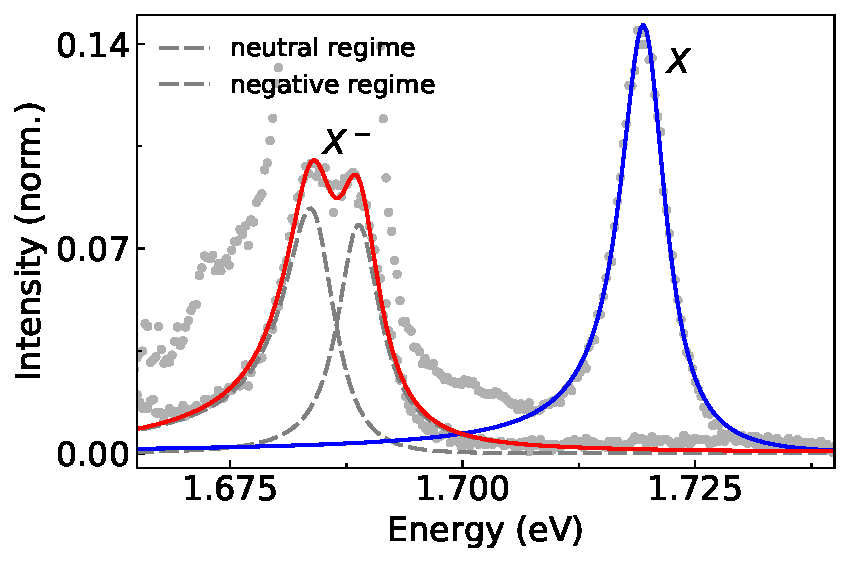
\includegraphics[height=0.65\textwidth]{X_Trion_fit}
	\end{subfigure}
	\begin{subfigure}{0.49\textwidth}
		\caption{}
		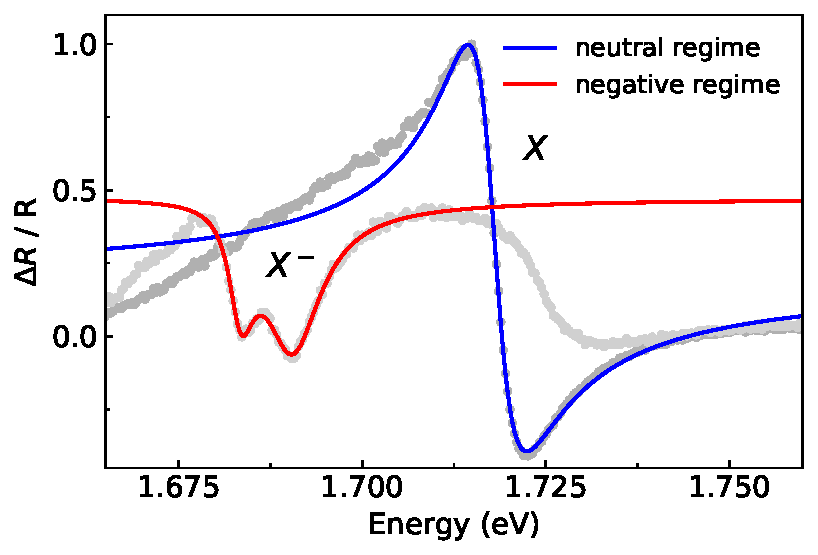
\includegraphics[height=0.65\textwidth]{RF_neut_neg}
	\end{subfigure}
	\caption{Fits of the exciton (X) and trion (X$^-$) features in a neutral and negatively charged spectrum. \textbf{A} \pl : The lineshape in the fitting model is a lorentzian with adaptive linewidth to model the slight asymmetry of the peaks. It is tuned with a sigmoid function, according to a symmetry parameter. The double-peak of the trion feature is a sum of two asymmetric lorentzians. \textbf{B} Reflection: The exciton resonance in this \hbng encapsulated sample does not show a clean dip and can be approximated by a model function corresponding to the scattering cross section of a fano resonance. The trion double dip can be fitted using a sum of two asymmetric lorentzians. However, in contrast to the \pl fit, a constant shifting parameter is added, and the starting values for the scaling parameter are chosen negative.}\label{linefits}
\end{figure}

To precisely quantify positions and linewidths of the spectral features, they have to be modelled using appropriate fitting functions. In \pl all peaks should ideally have a lorentzian line shape (see Figure \ref{plspectrum} \textbf{A}). 
\begin{align}
i(\nu)&= \frac{a}{1+\epsilon^2} \\
\epsilon &= \frac{\nu_0 - \nu}{\gamma /2}\label{lorentz}
\end{align}
where $I$ is the intensity, \epsilon is the reduced energy, composed of the energy $\nu$, the peak position $\nu_0$ the linewidth $\gamma$ at \textsc{fwhm}. For a maximum value $a$ of 1, the function is normalized. In the crowded spectrum of an imperfect sample however, this is only an approximation, as the different peaks blend together and can have fine structures, that cannot be resolved as individual features. This leads not only to a broadening of the lines, but also skews the line shape, mostly resulting in a ``red shoulder'' -- higher intensity towards the low-energy end of the peak. To accurately model these features and get good estimates for peak positions as well as linewidths the lorentzian has to be expanded. A generic way of modelling an asymmetric line, that is close to the ``natural'' linewidth is using a lorentzian with variable linewidth $\gamma$, meaning the static linewidth of in \ref{lorentz} is replaced by a smooth sigmoid function, that includes an additional symmetry parameter\cite{stancik_simple_2008}.
\begin{equation} \gamma = \frac{2\gamma_0}{1+e^{k(\nu-\nu_0)}}\label{asymlorentz} \end{equation}
This value is then insterted into \eqref{lorentz}. The symmetry parameter $k$ scales the steepness of the s-cuve sigmoid function and thus the skeewedness of the lineshape. The $\gamma_0$ parameter is identical to $\gamma$ at $\nu_0$ and corresponds to the peaks linewidth. For $k=0$ \eqref{lorentz} collapses to $\gamma_0$ and the standard lorentz lineshape is recovered. The asymmetric lorentzian can be used to model all peaks in the \pl spectrum.

In reflection spectroscopy, the signal should correspond to the absorption of the sample. Therefore the straight foreward way to model features would base on a lorentzian function as well, only with a negative sign\footnote{The sign of the fitting functions depends on the definition of the spectrum itself. In this work, the background is substracted from the signal, yielding the reflection off the flake. A flipped sign on the other hand corresponds to the absorption.}. However, in an \hbn-encapsulated sample, the spectrum can be more complicated (see Figure \ref{rfspectrum}). The neutral exciton resonance has a higly asymmetric lineshape, that cannot be modeled by a bare lorentzian (either \eqref{lorentz} or \eqref{asymlorentz}). A more general function is the lineshape of a fano resonace. The physical background is the interference between a resonance and a continuous background\cite{fano_effects_1961}. In case of encapsulated \tmdg monolayers, this lineshape stems from the \hbng layer, that forms a microcavity with the underlying reflective \si/\sio substrate\cite{scuri_large_2018}.
\begin{equation}
\frac{(q+\epsilon)^2}{(1+\epsilon^2)} = 1 + \frac{q^2+2q\epsilon-1}{1+\epsilon^2}\label{fano}
\end{equation}
where $q$ is the so-called fano parameter. This can be seen as a more general form of \eqref{lorentz}. For $q=0$ the shape of \eqref{fano} reduces to a downwards facing lorentzian. Just like for the trion and all \pl features, the linewidth parameter for \eqref{asymlorentz} can be deployed to skew the function to better fit real data.

The trion signal in the charged spectrum shows a double dip. While the physical process would demand a fano-type model just as for the neutral exciton, the close proximity of both signals and the strong background complicate the correct estimation of the peak position. Therefore a negative asymmetric loretzian is the naive but effective choice. To compensate for the strong background of the neutral resonance, a constant parameter is added, that gives the peaks a positive offset. 
Examples of the fitting process for reflection and \pl spectra can be seen in figure \ref{linefits}. To use the explained fitting functions, the data was sliced to isolate and fit each feature. This makes the minimum and maximum in the energy scale additional parameters that in practice strongly influence the convergence behaviour of the fitting algorithm. However, the disentanglement of the individal peaks makes it easier to finetune the models parameters, such that the most accurate estimate can be found.

\section{Ws\textup{e}$_2$ spectrum at different doping levels}

In all semiconductors the density of free charges through intentional or unitentional doping strongly influences its behaviour. \textsc{Tmd} samples very often exhibit unintentional doping\cite{kang_origin_2017, eshun_doping_2015}. Additionally other defects of different nature leave marks in the optical spectrum \cite{chow_defect-induced_2015,lin_defect_2016}. The discussion and interpretation of the spectrum thus becomes harder and highly speculative in samples prepared without control of the charge density. Gate-tunabillity therefore becomes a necessairy tool to establish a ground truth for a neutral sample but also to study the spectrum in charged environment intentionally.

\subsection{Photoluminescence spectrum}

\begin{figure}[t]
	\begin{subfigure}{0.49\textwidth}
		\caption{}
		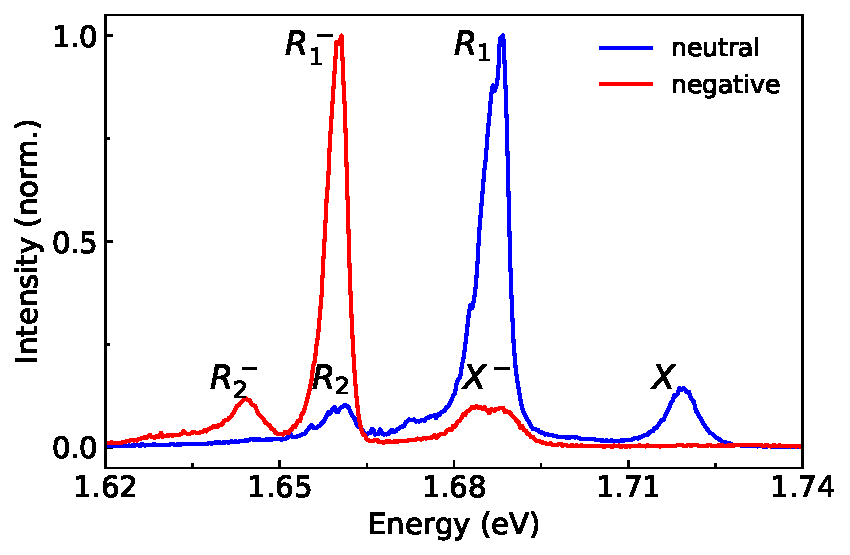
\includegraphics[height=0.65\textwidth]{spectrum_neutral_negative}
	\end{subfigure}
	\begin{subfigure}{0.49\textwidth}
		\caption{}
		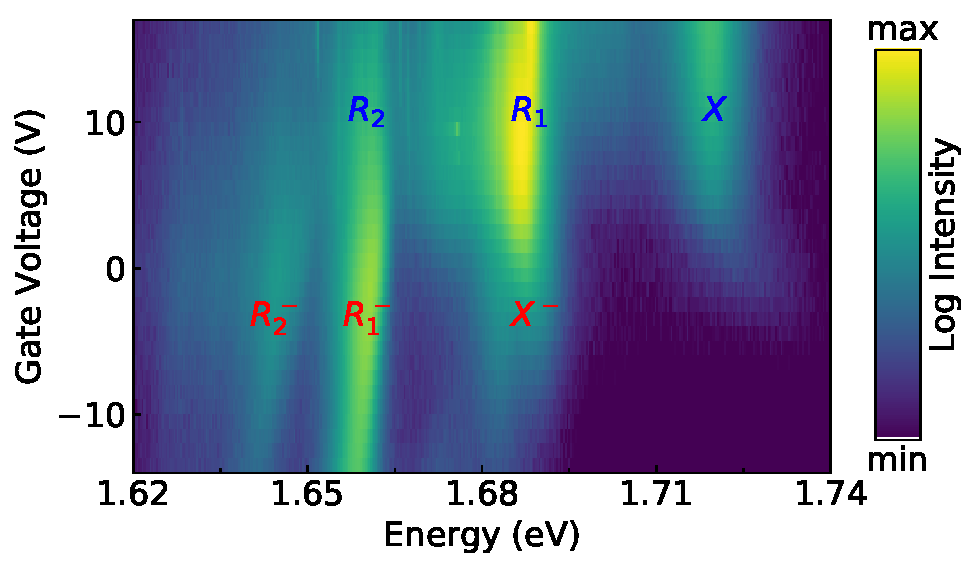
\includegraphics[height=0.65\textwidth]{Voltsweep}
	\end{subfigure}
	\caption{Photoluminescence of \wse at different doping levels. \textbf{A} Spectra in the neutral and negatively charged regime. The \pl of the exciton ($X$) is clearly visible at the blue end of the spectrum. The replica peaks ($R_1$, $R_2$) correspond to acoustic phonon sidebands of $Q$- and $K'$-indirect excitons with low-intensity features to the red indicating optical sidebands. In a negtively charged regime, they vanish in favor of redshifted peaks, that correspond to the trion (X$^-$) that is split by electron-electron exchange interaction, and its momentum indirect counterparts. While $R^-_1$ fits the picture as an accoustic sideband of $X^-$, $R^-_2$ seems to be the charged spin-unlike dark state. \textbf{B} Spectral features in a gate-sweep. The plot can be devided into a neutral and charged regime below and above 5V. This threshold is a signature of unintentional n-doping and varies across the sample.}\label{plspectrum}
\end{figure} 

\begin{figure}[t]
	\begin{subfigure}{0.49\textwidth}
		\caption{}
		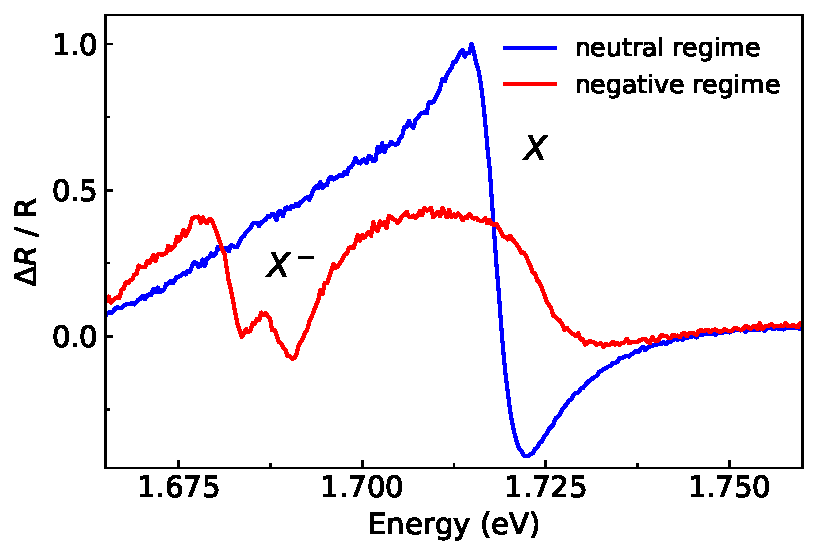
\includegraphics[height=0.65\textwidth]{RF_neut_neg_pure}
	\end{subfigure}
	\begin{subfigure}{0.49\textwidth}
		\caption{}
		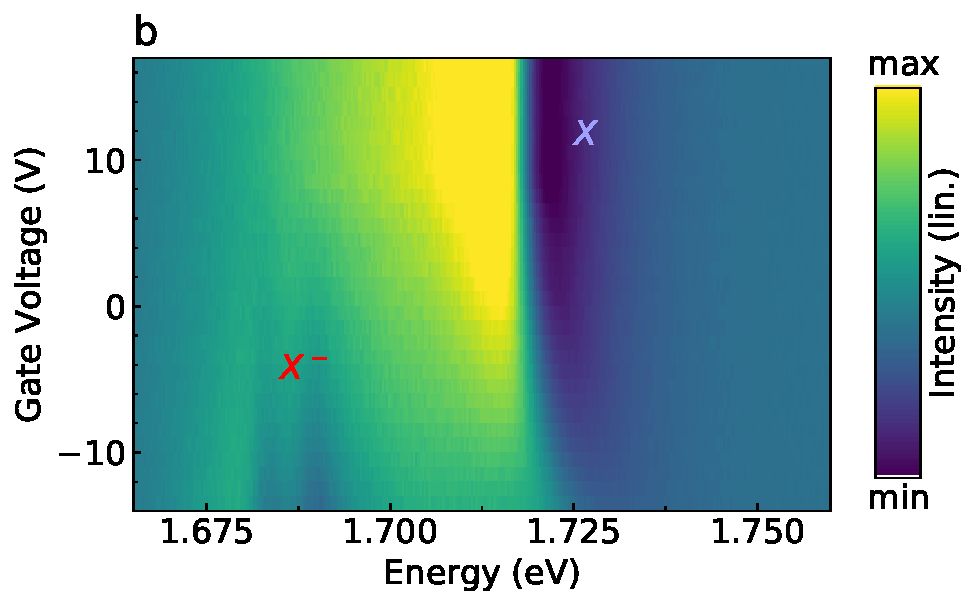
\includegraphics[height=0.65\textwidth]{RF_Voltsweep}
	\end{subfigure}

	\caption{Reflection of \wse at different doping levels. \textbf{A} The reflection spectrum of \wse in a neutral and negatively charged regime. The neutral spectrum shows a strong response, corresponding to the main exciton resonance (X). The absorption of the exciton almost vanishes in the charged spectrum and a double dip appears, that corresponds to the trion resonance, resolving the typical exchange splitting (X$^-$). \textbf{B} Reflection spectra at different voltages. The exciton absorption shows a similar response as in \pl, however stretched to lower voltages. The absorption at the trion resonance can be resolved much better, than the corresponding peaks in \pl. }\label{rfspectrum}
\end{figure}

The \pl spectrum is pictured in figure \ref{plspectrum} both in a neutral and charged regime. The sudden change in the spectrum at 5 V shows, that at this point on the sample, the \tmd-flake is negatively doped. As a result only the neutral and negative regime could be studied. The peak to the blue end of the spectrum belongs direct spin-like neutral exciton ($X$). This peak is well understood and can therefore be used to benchmark the spectral linewidth and the overall quality of the sample. With a linewidth of 6.8 meV the exciton is still above the intrinsic homogeneous linewidth which is reported to be below 2 meV\cite{moody_intrinsic_2015, ajayi_approaching_2017}. Inhomogeneous broadening can be mostly attributed to local changes in the potential landscape that can arise from defects, impurities as well as strain induced shifts in the band structure\cite{zhu_strain_2013}. The diffraction limited spot of the objective is large enough to cover a large ensemble of slightly different contributions to the \pl signal, that merge to a broad peak. Apart from the \textsc{fwhm} linewidth of the exciton peak, both a significant asymmetry parameter in the fit as well as a slight deviation from the lorentzian line-shape are indicators, that the feature has an considerable substructure and there is still room for improvement in terms of sample fabrication.

However, the linewidth-limited resolution of the present sample is good enough to distinguish the fine splitting of the trion peak in the charged regime ($X^-$). When the gate voltage is tuned, the Fermi level is shifted. The negative regime is reached when the Fermi level rises above the lower $K$ and $K'$ valleys in the conduction band and free charge carriers enter the flake. Optically excited excitons can bind electrons from either of the two valleys resulting in two a-priori degenerate trion states, that differ energetically because of a difference in Coulomb exchange interaction \cite{courtade_charged_2017}. The resulting splitting can be resolved in the present sample and has a value of 5.2 meV. The spectral difference to the exciton peak in the neutral regime gives an estimate of an additional trion binding energy. Taking into account the exchange splitting it has a value of 30.5 - 35.8 meV. Since the separation of the two trion peaks is quite low, the linewidth estimates from the fit are only a rough estimate but are close to the neutral exciton at 5-7 meV.

The peaks to the red in both the neutral and charged spectra can be explained using the phonon sideband model described in \ref{sidebands}. The $Q$-indirect exciton should lie above the direct spin-unlike state. Therefore it makes sense to identify the intense $R_1$ peak with its acoustic sidebands, putting the $Q$-exciton roughly 19 \pm 2 meV below $X$. The optical sidebands coincide with a low intensity bump that fits the predicted energies. The direct spin-unlike exciton ($D$) should be 40 meV to the red of $X$, but cannot be resolved clearly, possibly because $R_1$ is broad and intense enough to merge with the weak \pl of $D$. Its momentum-indirect counterpart in $K'$ should have the same energy, thus we can estimate its phonon sidebands, which fit the strong $R_2$ peak and the corresponding low-intensity feature to the red.

Assuming the nature of the phonon sidebands does not change fundamentally in a charged environment it is worth a try to treat the charged spectrum in a similar fashion. Analogous to the trion, the energy of the peaks should redshift upon interaction with free charge carriers. When shifting the $Q$-valley by the trion binding energy, it fits the two most intense replica peaks in the charged spectrum ($R^-_1, R^-_2$). However, $R^-_2$ also matches $D$ shifted by the trion binding energy. This could explain the relatively strong signal at this energy. The weak feature to the red could then charged acoustic replica of $K'$. 

\subsection{Reflection spectrum}

The reflection spectrum offers a way to quantify a materials absorption. In \tmds it can therefore offer a way to disentangle exciton resonances from states, that form by their non-radiative decay. These include the discussed phonon sidebands but also defect states and quantum dots, that have low absorption but brighten up trapped excitons\cite{srivastava_optically_2015}. The reflection spectrum therefore offers a more ``pure'' view on the direct exciton and the charged trion.
The reflection spectrum can be seen in figure \ref{rfspectrum}. The neutral spectrum shows a clear signature of the direct exciton resonance ($X$). This spectral feature in an \hbng encapsulated sample has the shape of a fano resonance, because of interference effects. The \tmd-\hbng heterostructure acts as a microcavity and shows very high reflectivity at the resonance frequency\cite{scuri_large_2018}. Upon tuning the gate to negative voltages, the absorption and reflection at the exciton resonance is suppressed and the trion resonance forms ($X^-$). Just like in \pl this resonance exhibits a splitting due to coulomb exchange energy. 


\section{Measuring the valley zeeman effect}

As described in section \ref{zeeman} the band gap and exciton energies in \tmds shift when exposed to an out-of-plane magnetic field. These shifts are reversed in light of opposite helicity and differ for different types of excitonic processes. Measuring the splitting, and quantifying it through the $g$-factor can yield a deeper insight in the nature of the spectral features. Figure \ref{waterfall} and \ref{waterfallRF} show the \pl and reflection spectra for different gate voltages at 0 and 8 T. Because of different magnetic shifts of the different peaks, looking at \sigma$^+$ and \sigma$^-$ polarized spectra at high magnetic field can help to resolve features, that are otherwise hidden by inhomogeneous broadening. The first interesting feature to study in this fashion is the two trion peaks ($X^-$). At 8 T they reveal significant change in their splitting, merging to one peak in \sigp while showing a clear splitting in \sigm. As will be discussed later on, this difference is so far unaccounted for but may be coupled to the asymmetry in intensity when the gate-voltage is swept.

The trion fine structure is a result of electron-electron exchange interaction. The singlet-state consists of an exciton and an electron of opposite spin at the $K$-point while the triplet state involves an additional electron in the $K'$-valley, but with the same spin component as the electron in the exciton. The spin-parallel triplet state has a lower binding energy, which allows to also observe the different behavior with regards to the charge density. At high negative gate voltages, both peaks are less intense with the blue peak losing signal much more rapidly. The reasons for that are speculative at best. Recent measurements in \ws point to the singlet state being stable only at low temperatures\cite{vaclavkova_singlet_2018}. Similarly, the triplet state in \wse could be more sensitive to large densities of free charge carriers. How this connects to their difference in magnetic moment is unclear.

\subsection{G-factors}

\begin{figure}[t]
	\begin{subfigure}{0.49\textwidth}
		\caption{}
		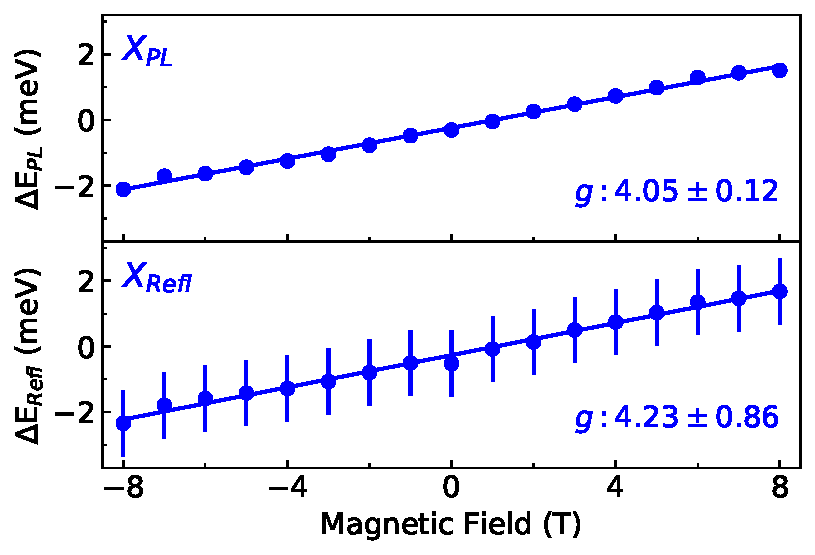
\includegraphics[width=\textwidth]{G_X}
	\end{subfigure}
	\begin{subfigure}{0.49\textwidth}
		\caption{}
		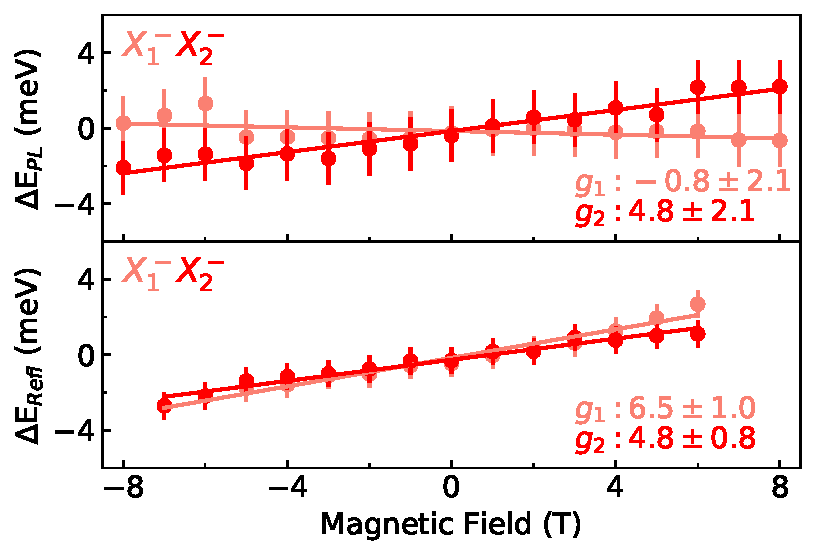
\includegraphics[width=\textwidth]{G_T}
	\end{subfigure}
	\caption{Exciton valley splitting in \pl and reflection. \textbf{A} The $g$-factor of the neutral exciton is in good agreement with previous studies. The fit of the reflection measurement has a large error bar, because of the complicated lineshape. Since the variance of the data points is low, this seems to be a systematic error. \textbf{B} The trion peak can only be reliably modeled in the reflection spectrum because of insufficient signal-to-noise ratio and limitations of the linewidth. The fits suggest a different $g$-factor for the two subfeatures.}
	\label{Xfits}
\end{figure}

\begin{figure}[t]
	\begin{subfigure}{0.49\textwidth}
		\caption{}
		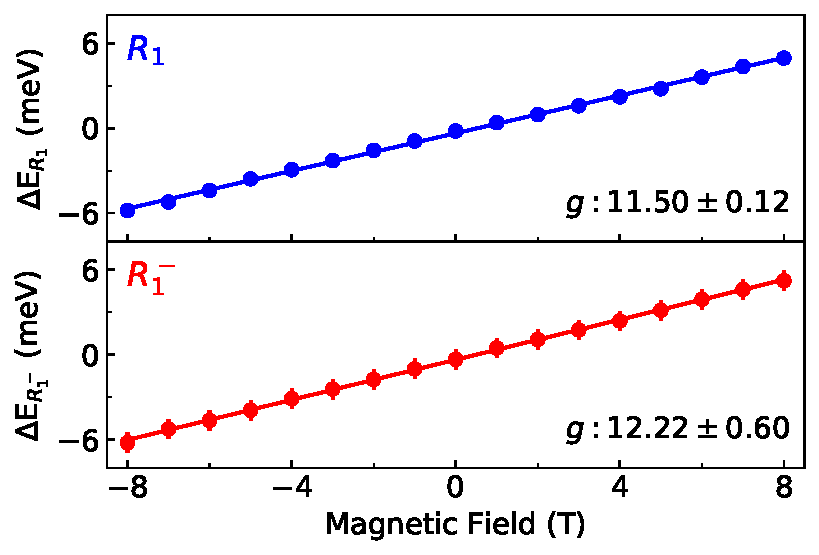
\includegraphics[width=\textwidth]{G_R1}
	\end{subfigure}
	\begin{subfigure}{0.49\textwidth}
		\caption{}
		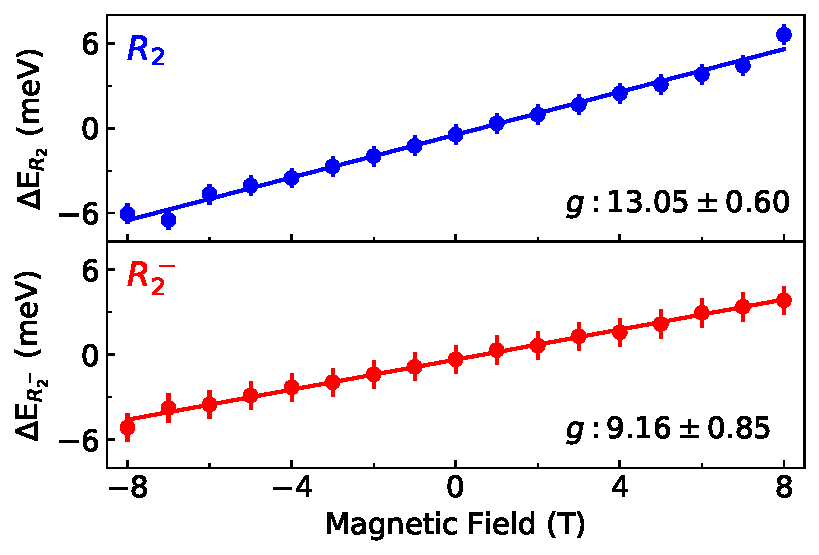
\includegraphics[width=\textwidth]{G_R2}
	\end{subfigure}
	\caption{Valley splitting of phonon replica. \textbf{A} The intense $R_1$ peak and its charged counterpart $R^-_1$ show a similar $g$-factor, suggesting the same origin. This is consistent with the proposed model, that identifies the peaks as acoustic sidebands of momentum-indirect excitons in the $Q$-valley. $R_1$ is of particular interest, because this feature conventionally is attributed to the trion. The strong difference in the $g$-factor however suggests a different origin than the trion feature, even though they share the same energy in the spectrum. \textbf{B} The neutral peak $R_2$ was previously identified as a phonon sideband of the $K'$-indirect exciton. The high $g$-factor however does not offer a direct argument to support this assumption. However, the charged counterpart $R^-_2$ has a similar $g$-factor as was previously measured for $D$, which underscores the assumption of the feature being the charged spin-unlike exciton in $K$. } 
	\label{Rfits}
\end{figure}

The magnetic splitting $\Delta E$ can be quantified by the $g$-factor. Because $\Delta E$ is linear in magnetic field strength $B$, the peak positions can be fitted using simple linear regression where the slope is connected to the $g$-factor in the following fashion:

\begin{align}
	g &=  \frac{1}{\mu_B}\underbrace{\frac{\Delta E}{\Delta B}}_{slope} \\
	\Delta E &= E_{\sigma^+} - E_{\sigma^-}
\end{align}

Because the splitting is a lot smaller than the linewidth---0.25 meV / T at a linewidth of 7 meV---the peaks have to be fitted using the procedures described in \ref{fits} to obtain a low error and therefore an accurate estimate for the $g$-factor. Not all features can be resolved well enough, because of either a bad signal to noise ratio or linewidth-related blending with other peaks.

The $g$-factor of the neutral exiton and trion resonances can be measured in both \pl and reflection spectroscopy (see figure \ref{Xfits}). This helps to cross-check experimental results. In case of the neutral exciton, both methods yield a $g$-factor that aligns well with many previous studies \cite{plechinger_excitonic_2016, stier_exciton_2016, srivastava_valley_2015, mitioglu_magnetoexcitons_2016}and also with each other. The fits of the reflection spectra carry a relatively high error. The error bars were estimated by eye using plots to determine deviation of the lineshape from the peaks maxima and minima. Because these errors are much higher than the standard deviation it is fair to say, that they only provide a coarse upper bound. They most likely origin from the substantial deviation of the lineshape from the ideal fano-resonance on the blue and red shoulder.

The trion resonance is much more easy to measure in reflection. The reason for this is partly the bad signal to noise ratio of its \pl signal, that can be linked to the longer lifetime of the charged state\cite{hao_trion_2017}. But another factor seems to be the limited resolution due to the linewidth of the peaks. The two peaks in the reflection spectrum are seperated by roughly 2 meV more, than in \pl. The reason for that could simply be the fact, that the lorentzian fit does not really reflect the proper lineshape in the reflection spectrum. Fitting the trion absorption with a double fano lineshape could possibly resolve this difference. For the calculation of the $g$-factor this should however not make a difference.

While the trion fits carry a significant error---also in reflection---they clearly show a different $g$-factor for each of its features. Since the decay of the trion leaves one free electron behind, it makes sense, that the trion features show the same $g$-factor as $X$. Nonetheless, this difference has also been observed in \ws samples at even higher magnetic fields, suggesting a non negligible influence of the excess electron towards the total magnetic moment\cite{plechinger_excitonic_2016}.

Having the uncertainty in mind we can compare the trion $g$-factor to the strong $R_1$ peak in the neutral spectrum (see figure \ref{Rfits}). Because it has the same energy as the trion, it is easy to misidentify both features as the same peak and attribute them to the trion. Especially if the sample has no gate control intrinsic electron doping offers a qualitative but not accurate argument for this identification. The magnetic field measuements however show a clear difference between their respective valley splitting. As stated the $g$-factor of the trion is hard to determine in \pl and has a large error. However, it is bound between 0 and around 6 which is half of the $g$-factor of $R_1$. The strong mismatch can also be observed qualitatively in \ref{waterfall}.

Unfortunately this leaves the question about the origin of the high $g$-factor of $R_1$. As briefly discussed in section \ref{zeeman} the momentum indirect exciton in $Q$ should not have a $g$-factor at all, when only looking at the orbital and spin contributions. The effective mass for electrons at the $Q$-point has however not been calculated for this thesis and therefore the theoretical model predicting the $g$-factor still has to be completed. This is similar for the $K'$ indirect exciton and the corresponding peak $R_2$, that should be composed of its accoustic phonon sidebands. When counting the oribital and spin contributions it should have the same $g$-factor as $X$. That this is not the case means, that a more thorough theoretical understanding is necessairy to verify or falsify the identification of the peak.

When looking at the charged spectrum the $g$-factor of $R_1^-$ matches that of $R_1$ within the 2\sigma-range. Because their distance in energy to $X$ and $X^-$ also fits it is reasonable to regard the peaks as neutral and charged version of the same momentum-indirect exciton in $Q$.

As discussed in the previous section the second peak $R_2^-$ energetically matches the spin-unlike but direct dark exciton $D$. Therefore it is no wonder, that this is reflected in the significantly smaller $g$-factor with respect to the phonon sideband peaks. While it is higher than the value predicted in section \ref{zeeman} it is close to what was reported for the neutral dark exciton\cite{robert_fine_2017}.

\section{Comparison to bilayer ws\textup{e}$_2$}

\begin{figure}[t]
	\begin{subfigure}{0.49\textwidth}
		\caption{}
		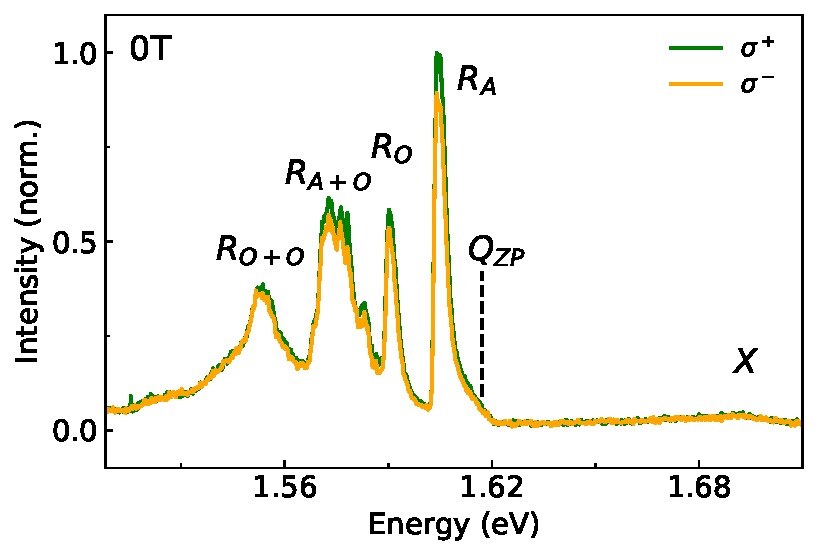
\includegraphics[height=0.65\textwidth]{bilayer_0T}
	\end{subfigure}
	\begin{subfigure}{0.49\textwidth}
		\caption{}
		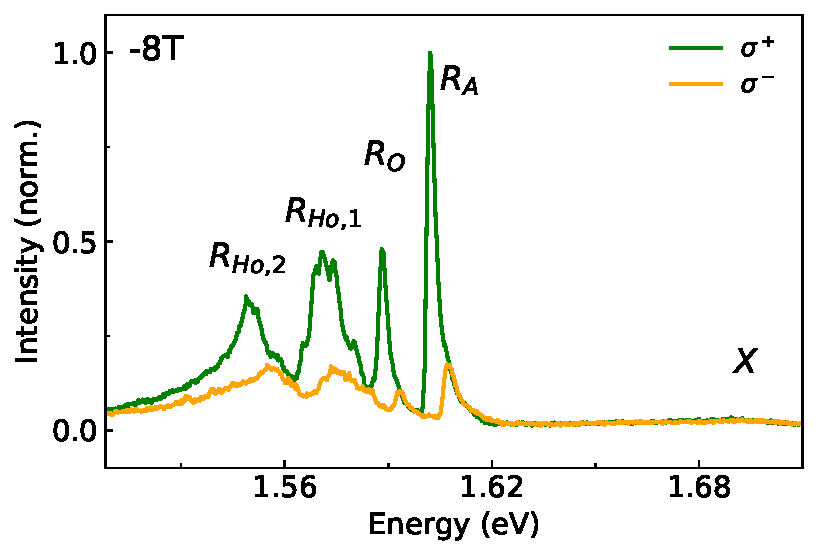
\includegraphics[height=0.65\textwidth]{bilayer_-8T}
	\end{subfigure}
	\caption{\textsc{Pl} spectrum of bilayer \wse at 0 and -8 T. \textbf{A} Because of the indirect band gap, the \pl spectrum is mostly composed of phonon sidebands of momentum-indirect excitons. When identifying the two blue peaks ($R_A$/$R_O$) as the accoustic and optical sidebands of $Q$, with the corresponding hole in $K$, the zero-phonon line $Q_{ZP}$ lies 73 meV below the direct transition $X$, that is shifted by around 36 meV with respect to the monolayer. \textbf{B} In a strong magnetic field the valleys split as they to in the monolayer, but the population of the excition states is "thermal", meaning they distribute according to Boltsman statistics with higher population in the low energy states. Because the spectral lines should all originate from the same underlying excitonic state, the intensity ratio between them does not shift in magnetic field.} 
	\label{bilayerthermal}
\end{figure}

\begin{figure}[t]
	\begin{subfigure}{0.49\textwidth}
		\caption{}
		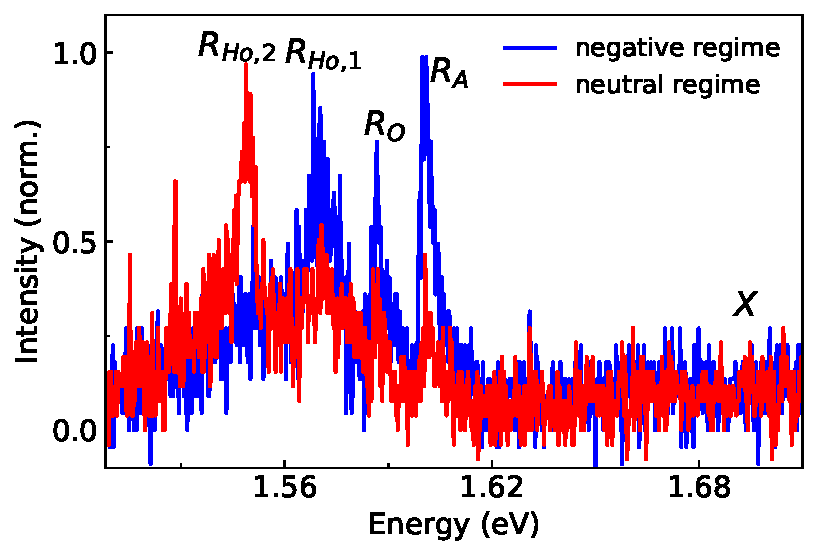
\includegraphics[height=0.65\textwidth]{BL_lowhigh}
	\end{subfigure}
	\begin{subfigure}{0.49\textwidth}
		\caption{}
		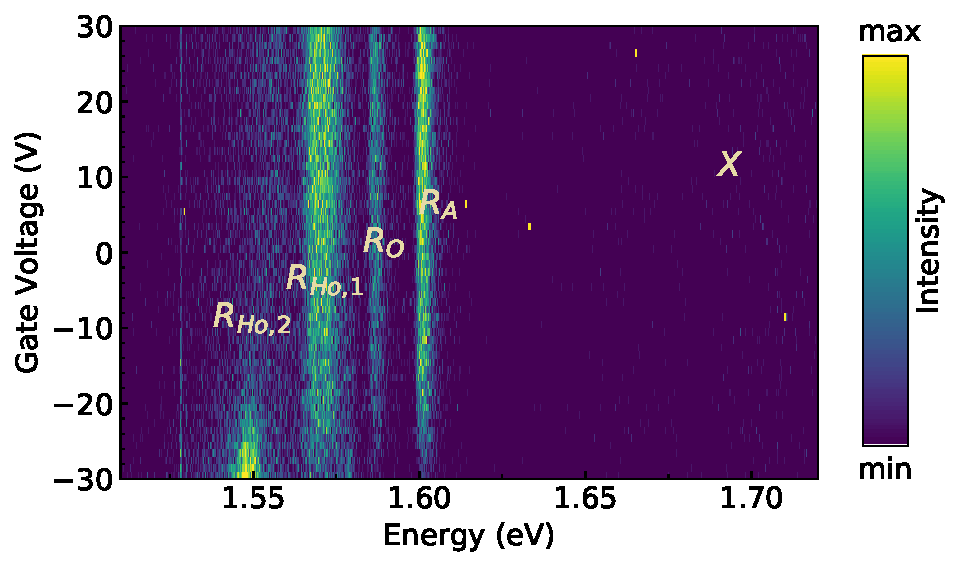
\includegraphics[height=0.65\textwidth]{BL_sweep}
	\end{subfigure}
	\caption{} 
	\label{bilayervoltsweep}
\end{figure}

\begin{figure}[t]
	\begin{subfigure}{0.32\textwidth}
		\caption{}
		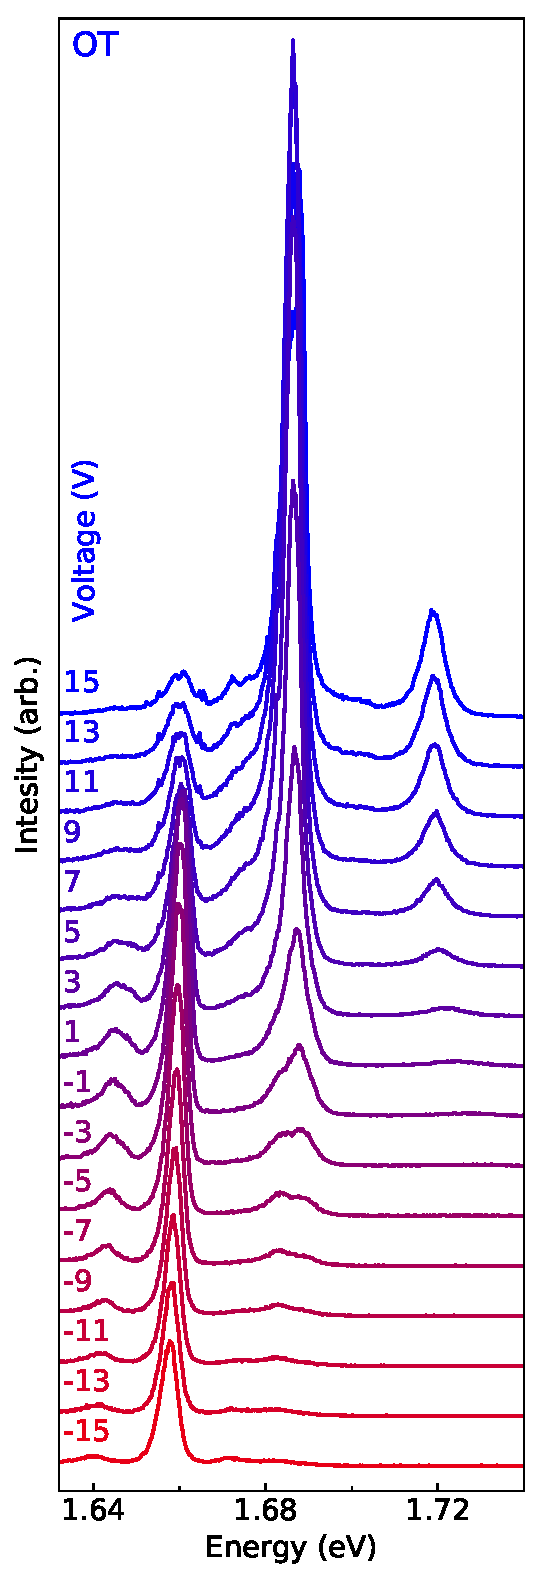
\includegraphics[width=\textwidth]{waterfall_0T}
	\end{subfigure}
	\begin{subfigure}{0.32\textwidth}
		\caption{}
		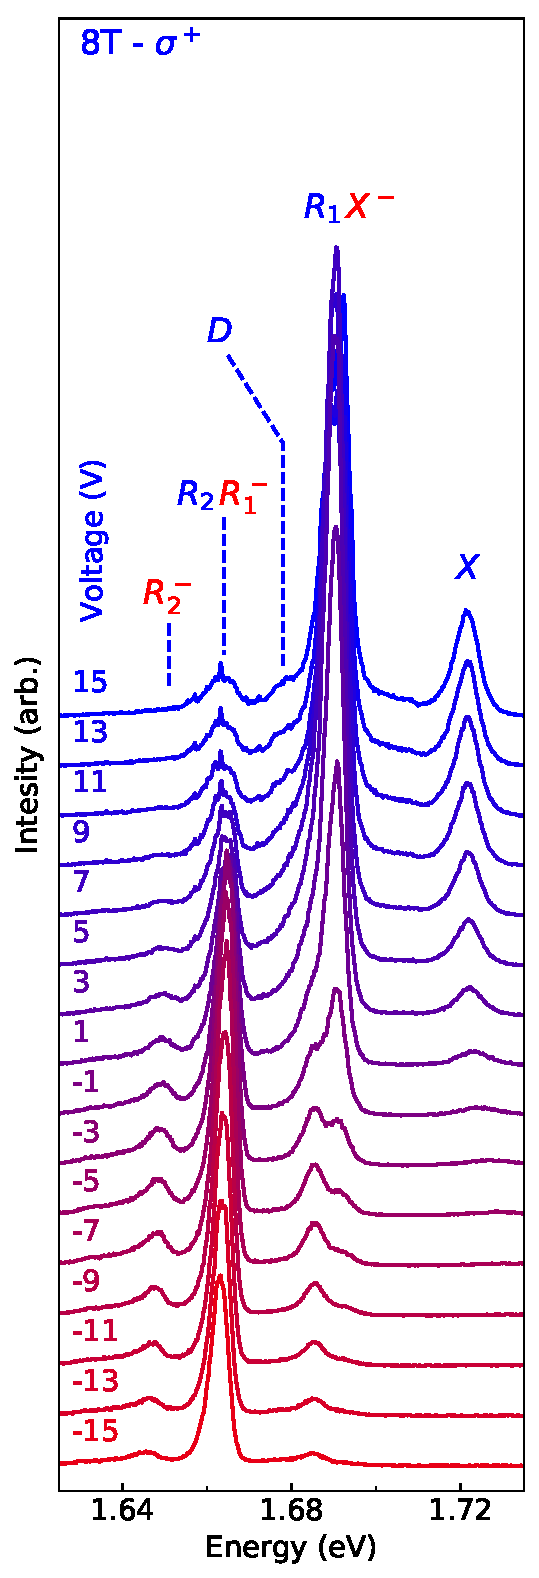
\includegraphics[width=\textwidth]{waterfall_8T_sp}
	\end{subfigure}
	\begin{subfigure}{0.32\textwidth}
		\caption{}
		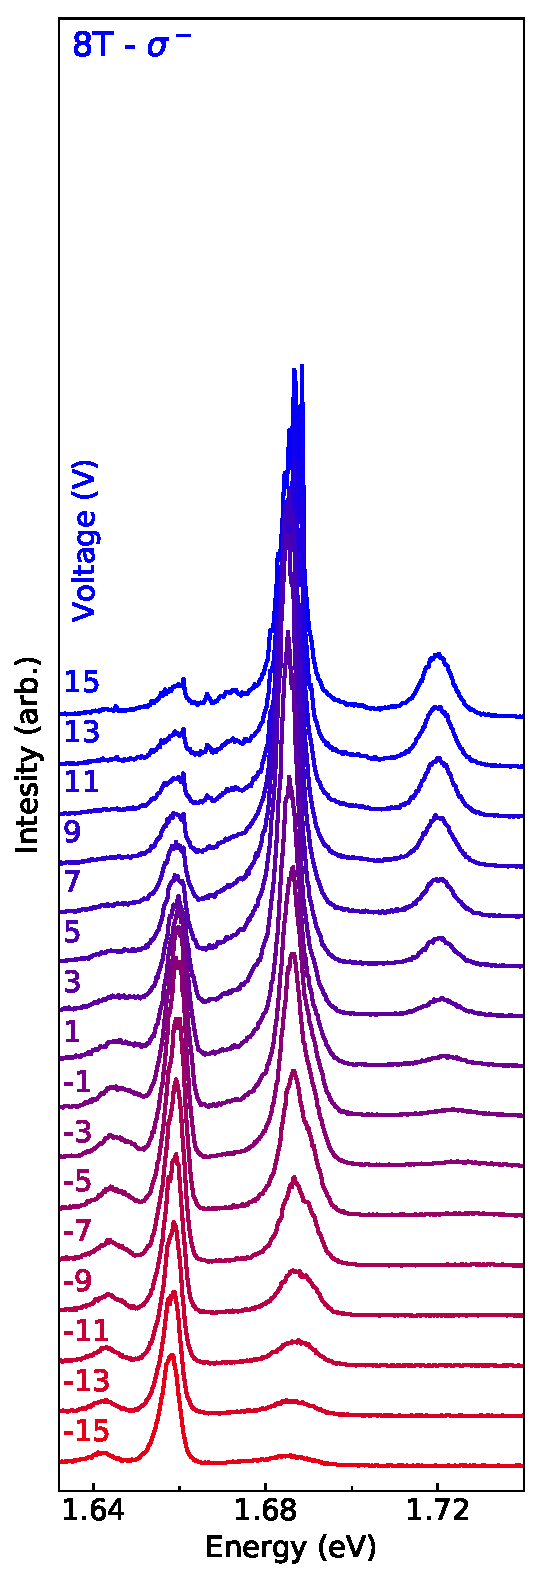
\includegraphics[width=\textwidth]{waterfall_8T_sm}
	\end{subfigure}
	\caption{\pl spectra of \wse at high magnetic fields for different gate voltages. In the neutral spectrum the dark exciton ($D$) lies to close to the strong phonon sideband $R_1$ to be resolved clearly. The strong splitting of this feature reveals $D$ more clearly in the \sigma$^+$-polarized spectrum at 8T (\red{gfactor}). The trion peak in the negative regime is composed of at least two features. As can be seen these peaks have different $g$-factors as well, that lead to a wide split in \sigma$^+$ and merge to one feature in \sigma$^-$.}\label{waterfall}
\end{figure}

\begin{figure}[t]
	\begin{subfigure}{0.32\textwidth}
		\caption{}
		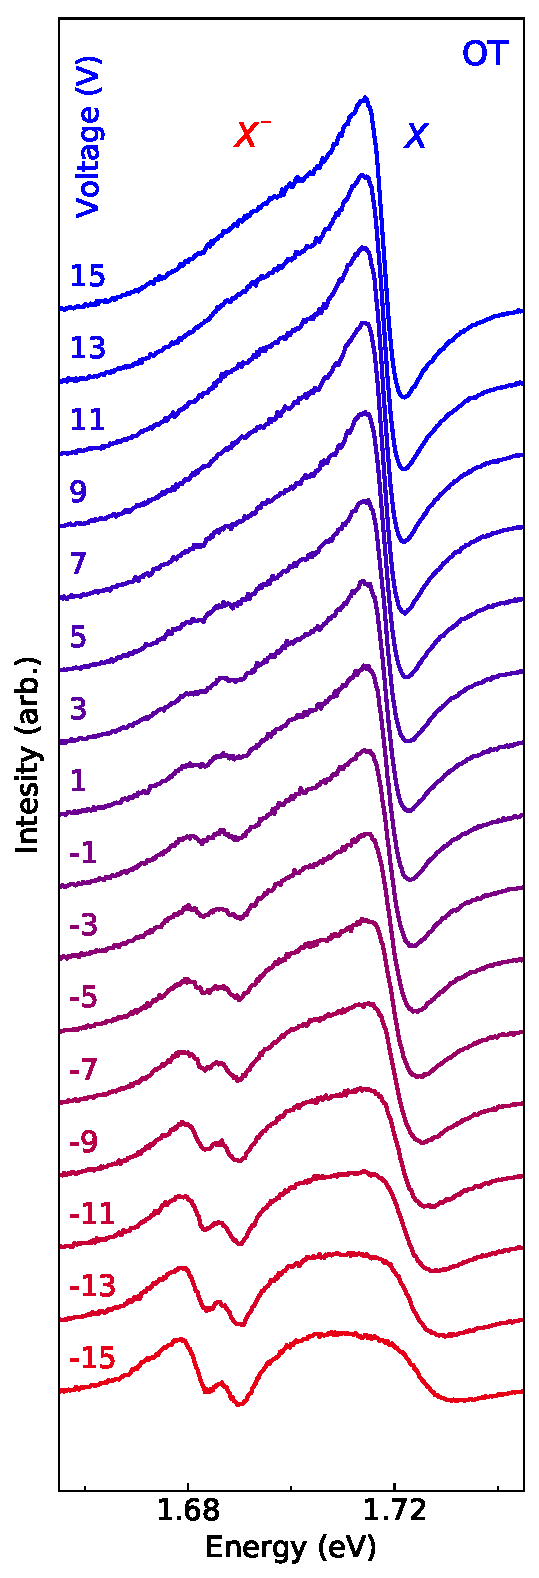
\includegraphics[width=\textwidth]{waterfall_0TRF}
	\end{subfigure}
	\begin{subfigure}{0.32\textwidth}
		\caption{}
		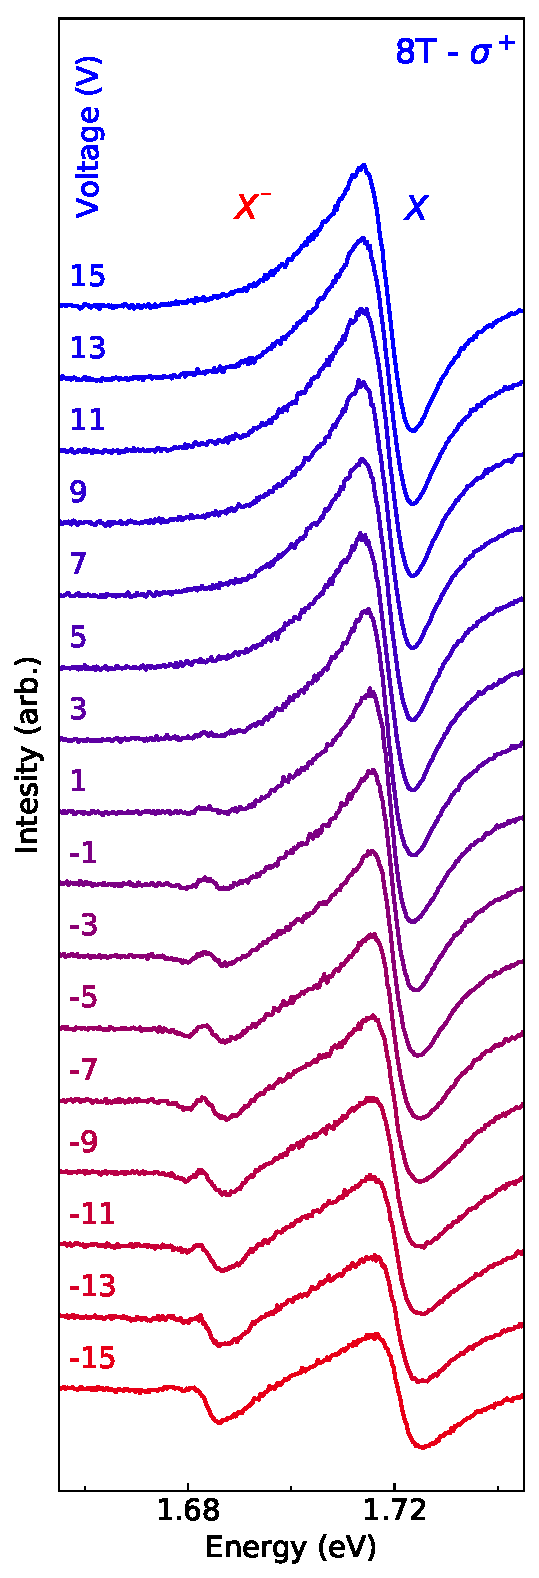
\includegraphics[width=\textwidth]{waterfall_8TRF_sp}
	\end{subfigure}
	\begin{subfigure}{0.32\textwidth}
		\caption{}
		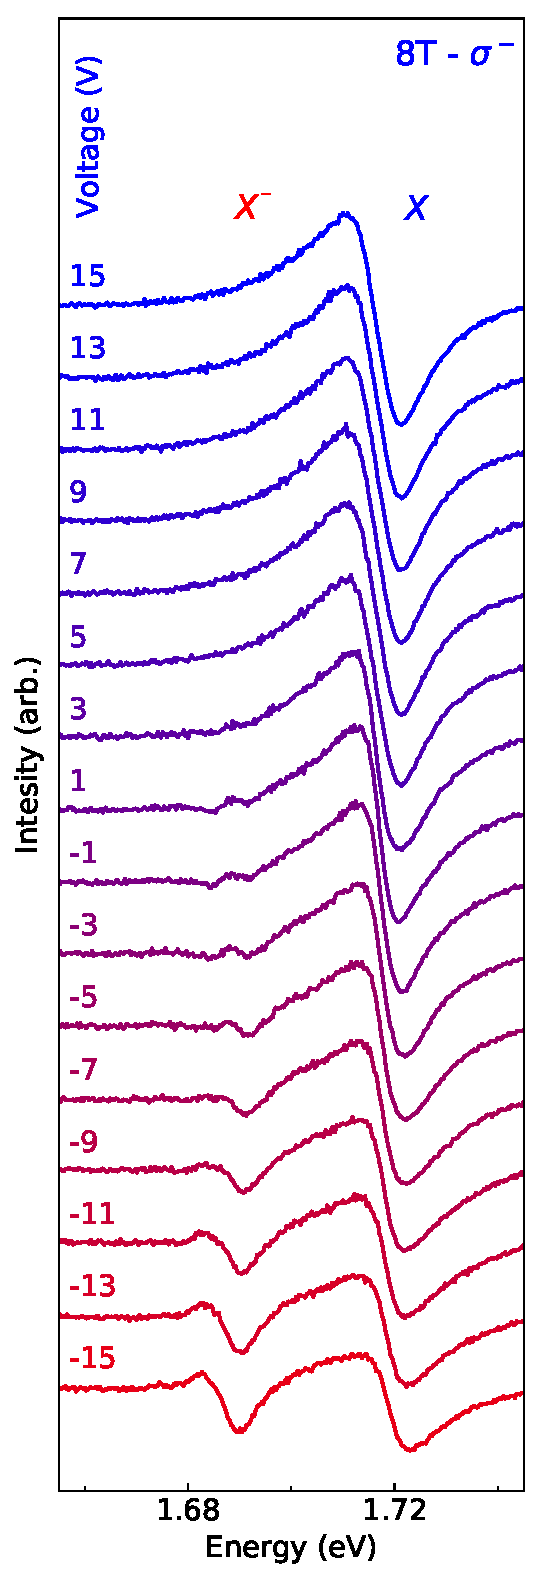
\includegraphics[width=\textwidth]{waterfall_8TRF_sm}
	\end{subfigure}
	\caption{\pl spectra of \wse at high magnetic fields for different gate voltages. In the neutral spectrum, towards the positive end, the replica peaks $R_1$ and $R_2$ get significantly skewed at 8 T, pointing towards several underlying peaks with different $g$-factors. The trion peak in the negative regime is composed of at least two features. As can be seen these peaks have different $g$-factors as well, that lead to a wide split in \sigma$^+$ and merge to one feature in \sigma$^-$.}\label{waterfallRF}
\end{figure}

As pointed out in section \ref{bilayer_theory}, bilayer \wse has an indirect band gap and most of the weaker \pl can be attributed to the decay of momentum-indirect excitons.
